\documentclass{scrartcl}
\usepackage[utf8]{inputenc}
\usepackage{hyperref}
\usepackage{url}
\usepackage[numbers]{natbib}
\usepackage{graphicx}
\usepackage{float}
\usepackage{array}
\usepackage{booktabs}
\usepackage{tikz}
\usetikzlibrary{positioning, backgrounds, arrows.meta}
\usepackage{cleveref} % this must be the last package to be loaded

\newcommand{\emailaddr}[1]{\href{mailto:#1}{\texttt{#1}}}

\title{\LARGE
    Distributed Lupus in Fabula\\
    A Replicated Real-Time Multiplayer Game Platform
}
\subtitle{Final Report for the Distributed Systems Course --- A.Y. 2025/2026}

\author{
    Leonardo Vorabbi \\ \emailaddr{leonardo.vorabbi@studio.unibo.it}
    \and
    Jacopo Bonifazi \\ \emailaddr{jacopo.bonifazi@studio.unibo.it}
    \and
    Alexandru Nicolescu \\ \emailaddr{alexandru.nicolescu@studio.unibo.it}
}

\date{\today}

\begin{document}

\maketitle

\begin{abstract}
    This report describes the design, implementation, and deployment of
    \emph{Distributed Lupus in Fabula}, a web-based, real-time multiplayer
    implementation of the social deduction game known as
    \emph{Werewolf} (\emph{Lupus in Fabula}).
    %
    Players join game rooms from their browsers, chat with each other
    (through role-restricted channels, such as a private night chat reserved
    for wolves), and play through the classic day/voting/night loop with
    hidden roles (villagers, wolves, and a seer), while the platform keeps
    every participant's view of the game synchronised in real time.

    The system is designed as a horizontally scalable distributed platform:
    a pool of stateless backend replicas (FastAPI + Socket.IO) serves
    WebSocket connections behind a reverse proxy / ingress load balancer,
    while the authoritative game state lives in a shared Redis store.
    %
    Cross-replica event propagation relies on Redis Pub/Sub with
    sender-based deduplication, so that players connected to different
    replicas observe the same game events.
    %
    From the players' standpoint, fault tolerance is most visible on
    disconnection: when a participant drops, the match is automatically paused
    and its state preserved, resuming as soon as the player reconnects (to any
    replica) or after a bounded grace period elapses.
    %
    Underneath, since Pub/Sub delivery is at-most-once, the platform layers several
    fault-tolerance mechanisms on top of it: publish retries with exponential
    back-off, automatic reconnection with channel re-subscription, a periodic
    anti-entropy loop that re-broadcasts authoritative state snapshots, a
    distributed sweeper that recovers phase timers scheduled by crashed
    replicas, and atomic state updates (optimistic transactions and
    \texttt{SET NX} locks) that prevent lost updates and duplicated
    phase transitions.

    The platform is containerised with Docker and deployable both via
    Docker Compose and on Kubernetes, where a HorizontalPodAutoscaler scales
    the backend between 2 and 8 replicas, rolling updates guarantee
    zero-downtime deployments, and a Prometheus + Grafana stack provides
    observability over WebSocket, Pub/Sub, and infrastructure metrics.
    %
    Correctness under replication is validated by dedicated multi-instance,
    reconnection, and distributed-safety test suites in addition to unit
    tests of the game logic.
\end{abstract}

\section*{Disclaimer}

During the preparation of this work, the authors used LLM-based tools
(Claude) to assist with the drafting of this report, code review,
and the refinement of infrastructure configuration files.

After using this tool/service,
the authors reviewed and edited the content as needed
and take full responsibility for the content of the final report/artifact.

\section{Concept}\label{concept}

\subsection{Type of product}

The project delivers a \textbf{web application} composed of two artifacts:

\begin{itemize}
  \item a browser-based \emph{single-page application} (SPA) acting as the
  graphical client, usable from any modern browser on desktop or mobile
  devices, with no installation required;

  \item a set of replicated \emph{web services} (the game backend) exposing a
  small REST API (health checks, lobby browsing) and a bidirectional
  event-based interface (Socket.IO over WebSocket, with HTTP long-polling as
  fallback) for real-time gameplay.
\end{itemize}

The two are complemented by an infrastructure layer (reverse proxy / ingress,
shared in-memory store, monitoring stack) that is part of the deliverable and
is described in \cref{infrastructure}.

\subsection{Use case}

The software implements \emph{Lupus in Fabula} (also known as
\emph{Werewolf} or \emph{Mafia}), a turn-based social deduction game.
%
A group of 5 or more players is secretly split into two factions:
\emph{wolves}, who eliminate one villager per night, and \emph{villagers}
(possibly including a \emph{seer}, who can privately inspect one player's
faction each night), who try to identify and lynch the wolves through a
public vote.
%
The game alternates \emph{day} (discussion), \emph{voting} (public lynching),
and \emph{night} (secret wolf and seer actions) phases, each bounded by a
timer, until one faction wins.

\begin{description}
  \item[What.] The platform hosts multiple concurrent \emph{game rooms}.
  Within a room, players chat in real time, configure the match (number of
  wolves and seers), declare themselves ready, and then play through the
  game loop. The server is authoritative: it assigns hidden roles, collects
  votes and night actions, advances phases when timers expire, computes
  eliminations, and detects the winning condition.

  \item[Where.] Players are geographically dispersed: the whole point of an
  \emph{online} version of a tabletop party game is letting friends play
  from different places. Each player only needs a browser and an Internet
  connection; the service itself runs in a datacenter (a container
  orchestration cluster).

  \item[When and how frequently.] Interaction is \emph{session-based} and
  highly interactive: a match lasts tens of minutes, during which every
  player continuously exchanges events with the system (chat messages,
  votes, phase updates) with soft real-time expectations --- an
  elimination or a phase change must be perceived (nearly)
  simultaneously by every participant.

  \item[How, and on which devices.] Users interact exclusively through the
  web GUI (Vue.js SPA) over a persistent Socket.IO connection. No dedicated
  client is needed, which maximises reachability and lowers the entry
  barrier for casual players.

  \item[Data.] The system stores only \emph{ephemeral game state}: room
  snapshots, player registries (nickname, host flag, readiness,
  connectivity), secret role assignments, votes, night actions, and phase
  timers. This state is kept server-side in a shared Redis store --- clients
  are never trusted with authoritative data (a client that knew the role
  assignments could cheat). State expires automatically (TTL) hours after
  the last update, so no long-term personal data is persisted; players are
  identified by self-chosen nicknames, and no account or authentication
  infrastructure is required.

  \item[Roles.] Two role dimensions coexist. At the \emph{platform} level, a
  room distinguishes the \textbf{host} (who configures the match, can kick
  players, start the game, and restart it once ended) from regular
  \textbf{players}; the host role migrates automatically if the current
  host disconnects. At the \emph{game} level, players are secretly assigned
  the \textbf{wolf}, \textbf{seer}, or \textbf{villager} role, each with
  different visibility over the game state (e.g.\ wolves see each other's
  votes; the seer receives private inspection results).
\end{description}

\subsection{Why distribution is needed}

Following the classic motivations for distribution~\cite{ghosh2014distributed,
tanenbaum2017distributed}, several apply directly to this project:

\begin{description}
  \item[Inherent geographical distribution.] The problem itself is
  distributed: players sit at different machines in different places, and
  the functionality to provide (\emph{collaboration}, i.e.\ real-time shared
  play) implies communication across a network. A non-distributed version
  of this product simply cannot exist.

  \item[Fault tolerance and availability.] A match is a long-lived,
  stateful, social activity: a server crash that destroys every running
  game is far more costly than in a request/response application, because
  it disrupts groups of users simultaneously and the lost state (roles,
  votes, round progress) cannot be reconstructed by clients. The
  architecture therefore replicates the service tier: any backend replica
  can serve any room, because state is externalised to a shared store.
  The failure of a replica only forces its clients to reconnect (to a
  surviving replica), not to lose the match (\cref{fault-tolerance}).

  \item[Scalability.] The workload is connection-bound: every player holds
  a persistent WebSocket, and rooms are mutually independent. This makes
  the service embarrassingly parallel across rooms and thus a natural fit
  for \emph{horizontal scaling}: adding replicas increases the number of
  concurrently sustainable connections and rooms. In the Kubernetes
  deployment, an autoscaler adjusts the number of replicas to the load
  (\cref{availability}).

  \item[Resource sharing.] All replicas share the same infrastructure
  resources --- most notably the Redis store holding the authoritative game
  state and acting as the inter-replica message bus --- so that the
  \emph{same} logical room can be served by \emph{different} physical
  replicas transparently.
\end{description}

Distribution is therefore not an implementation whim but a direct consequence
of the use case; its price --- partial failures, message loss, concurrent
updates, and the impossibility of relying on a single global clock~\cite{lamport1978time} ---
is what most of the design in \cref{design} is about.

\section{Requirements Elicitation and Analysis}\label{requirements}

\subsection{Glossary}

\begin{description}
  \item[Room (or lobby)] An independent game session, identified by a
  user-chosen code, hosting one match at a time.
  \item[Host] The player who administers a room: configures the match,
  starts it, kicks players, and restarts the game once it has ended.
  \item[Phase] A stage of the game loop: \textsc{lobby}, \textsc{day},
  \textsc{voting}, \textsc{night}, \textsc{ended}.
  \item[Role] The secret game faction assigned to a player: \emph{wolf},
  \emph{seer}, or \emph{villager}.
  \item[Replica (or instance)] One of the interchangeable backend server
  processes serving client connections.
  \item[Snapshot] The complete, authoritative representation of a room's
  state, as stored server-side and sent to (re)connecting clients.
\end{description}

\subsection{Functional requirements}

Each requirement is followed by its \emph{acceptance criterion} (AC).

\begin{description}
  \item[FR1 --- Room creation and joining.] A user can create or join a room
  by choosing a nickname and a room code; the first user entering a room
  becomes its host. \emph{AC: two users entering the same code end up in the
  same lobby; exactly one host exists, even if two users join a new room
  simultaneously.}

  \item[FR2 --- Lobby browsing.] A user can list the currently open rooms
  (those still in \textsc{lobby} phase) with their host and player count.
  \emph{AC: a room in progress or ended does not appear in the list; an open
  room appears regardless of which replica serves the request.}

  \item[FR3 --- Match configuration.] The host, and only the host, can
  configure the number of wolves and seers while in \textsc{lobby}.
  Configurations that break the game balance are rejected (at least 5
  players, at least 1 wolf, at least 1 plain villager left).
  \emph{AC: a non-host attempt or an invalid configuration is refused with
  an error message; a valid change is visible to all lobby members.}

  \item[FR4 --- Readiness and game start.] Players declare themselves ready;
  the host can start the match only when all connected players are ready
  and the configuration is valid. \emph{AC: a start request with a
  non-ready player is rejected; on start, every player receives their
  secret role.}

  \item[FR5 --- Secret role assignment.] At game start the system randomly
  assigns roles according to the configuration; each player learns
  \emph{only} their own role (wolves also learn their teammates).
  \emph{AC: no message delivered to a villager's client ever contains
  another player's role before game end.}

  \item[FR6 --- Game loop and timers.] The game alternates
  \textsc{day} $\to$ \textsc{voting} $\to$ \textsc{night} phases, each
  bounded by a server-side timer; when the timer expires the phase advances
  automatically for everyone. \emph{AC: phases advance without any client
  input; all clients converge on the same phase and deadline.}

  \item[FR7 --- Public vote.] During \textsc{voting} every living player can
  vote a living target (or skip); votes are public, ties or skip-majority
  cause no elimination; the most-voted player is eliminated and their role
  revealed. \emph{AC: dead or disconnected players cannot vote; the tally
  matches the recorded votes even when voters are connected to different
  replicas.}

  \item[FR8 --- Night actions.] During \textsc{night}, wolves privately
  agree on a victim (seeing each other's votes), and the seer privately
  inspects one player's faction. \emph{AC: night choices are never visible
  to other players; the seer's result is delivered only to the seer, even
  if connected to a different replica than the one computing it.}

  \item[FR9 --- Win detection.] The system detects the end of the game as
  soon as a faction wins (no wolves left, or wolves $\geq$ non-wolves) ---
  including when the decisive event is a player abandoning the match ---
  and reveals all roles. \emph{AC: the ended screen shows winner and roles
  to every player; no further game action is accepted.}

  \item[FR10 --- Chat.] Players in a room can exchange real-time chat
  messages; system announcements (e.g.\ a player fleeing mid-game) appear
  in the same feed. \emph{AC: a message sent by a player connected to
  replica $A$ is received by players connected to replica $B$.}

  \item[FR11 --- Reconnection.] A player who loses the connection mid-game
  can rejoin the same room with the same nickname and receive the current
  authoritative state (including their role). \emph{AC: after a page
  reload during a match, the player sees the current phase, timer, and
  their own role.}

  \item[FR12 --- Host migration.] If the host disconnects, another
  connected player is automatically promoted host. \emph{AC: the lobby
  never remains without a host while at least one player is connected.}

  \item[FR13 --- Room administration.] The host can kick a player from the
  lobby, and can restart a finished game bringing everyone back to the
  lobby (with roles, votes, and readiness reset, and disconnected players
  cleaned up). \emph{AC: a kicked player is removed from every registry
  and notified; after restart, no ``ghost'' player remains and nobody is
  marked ready.}

  \item[FR14 --- Access control to running games.] A user who is not part of
  a match cannot join a room where a game is in progress or ended, and a
  nickname already connected to a room cannot be reused concurrently.
  \emph{AC: the connection is refused with an explanatory message.}
\end{description}

\subsection{Non-functional requirements}

\begin{description}
  \item[NFR1 --- Replication transparency.] Clients must not know, or care,
  which backend replica serves them: any replica must be able to serve any
  room, and two players in the same room must be able to play together
  while connected to different replicas. \emph{AC: the multi-instance test
  suite passes with 2+ replicas behind the load balancer.}

  \item[NFR2 --- Fault tolerance.] The crash of a single backend replica
  must not destroy any running match: affected clients reconnect and
  resume within seconds; matches served by other replicas must not be
  affected at all. Phase progression must not depend on the survival of
  the replica that scheduled the current phase timer. \emph{AC: killing
  one replica during a match, the game reaches its natural end.}

  \item[NFR3 --- Convergence (eventual consistency).] All clients of a room
  must converge to the same authoritative game state: temporarily missed
  events (e.g.\ during a network blip) must be repaired automatically
  within seconds, without user intervention. \emph{AC: a client that missed
  a broadcast converges to the authoritative snapshot within one
  anti-entropy period ($\sim$10\,s).}

  \item[NFR4 --- Safety of game rules.] Game-rule invariants must hold
  despite concurrency and replication: no lost updates on shared state, at
  most one host per room, at most one phase advancement per deadline (no
  double eliminations). \emph{AC: the distributed-safety test suite
  passes with concurrent clients on multiple replicas.}

  \item[NFR5 --- Scalability.] Capacity (concurrent connections/rooms) must
  grow by adding backend replicas, with no code changes and no
  single-replica bottleneck in the service tier; the deployment must
  support automatic horizontal scaling. \emph{AC: under load, the
  autoscaler increases replicas and new connections are spread across
  them.}

  \item[NFR6 --- Soft real-time interactivity.] Game events must reach all
  players of a room with sub-second perceived latency under nominal load.
  \emph{AC: load tests report end-to-end event fan-out latencies well
  below 1\,s at the target load.}

  \item[NFR7 --- Observability.] Operators must be able to inspect the
  health and behaviour of every component (connections per replica,
  Pub/Sub traffic, error rates, resource usage) through metrics,
  dashboards, and alerts. \emph{AC: Grafana dashboards display per-replica
  WebSocket and Redis metrics; alert rules fire on component failure.}

  \item[NFR8 --- Zero-downtime updates.] Deploying a new backend version
  must not interrupt the service. \emph{AC: a rolling update completes
  with no failed health checks and no window with zero ready replicas.}
\end{description}

\subsection{Implementation requirements}

By design (\cref{design}) the system needs an asynchronous, WebSocket-capable
service runtime, a shared low-latency store with publish/subscribe
capabilities, and reproducible containerised deployment. The concrete
constraints below descend from those needs plus course/administrative
context:

\begin{description}
  \item[IR1] The system shall be containerised and runnable both with
  Docker Compose (local, single machine) and on Kubernetes (cluster),
  since deployment automation and orchestration are learning goals of the
  project. \emph{AC: both \texttt{docker compose up} and the provided
  Kubernetes manifests bring up the full platform.}

  \item[IR2] The backend shall expose Prometheus-compatible metrics, as
  Prometheus + Grafana is the de-facto standard open-source monitoring
  stack and fits the zero-budget constraint. \emph{AC: \texttt{/metrics}
  is scraped successfully by the provided Prometheus configuration.}

  \item[IR3] Only free / open-source components shall be used (no managed
  cloud services), for economic reasons and local reproducibility on
  student machines. \emph{AC: the whole platform runs on a laptop via
  minikube.}
\end{description}

Programming languages and frameworks (Python/FastAPI, Vue.js, Redis) were
\emph{not} imposed a priori; they emerge as consequences of the design and
are motivated in \cref{implementation}.

\subsection{Relevant Distributed System Features}
\label{ds-features}

We now assess which classic distributed-system
concerns~\cite{tanenbaum2017distributed} are relevant for this project, and
to what extent.

\begin{description}
  \item[Transparency --- central.] \emph{Replication} and \emph{access}
  transparency are the core of the project: users must perceive a single
  logical game server, while requests and connections are actually served
  by interchangeable replicas (NFR1). \emph{Failure} transparency is
  pursued for server-side faults (a replica crash appears to the user as a
  brief reconnection, not as a lost match --- NFR2). \emph{Location}
  transparency is provided by naming services and virtual hosts (clients
  address \texttt{game.local}, never a specific pod). Migration,
  relocation, and persistence transparency are not relevant: components do
  not move at runtime and no long-term persistence is exposed to users.

  \item[Fault tolerance / dependability --- central.] The service tier must
  tolerate crash failures (fail-stop model) of any single replica, and
  temporary unavailability of the message bus. Uninterrupted service is
  required at match granularity: losing a running match is the failure to
  avoid. Recovery must be fast (seconds), since matches are paced by
  timers. Byzantine behaviour of \emph{servers} is out of scope (all
  replicas are trusted, deployed from the same image); malicious
  \emph{clients} are considered only at the game-rule level (a client must
  not be able to cheat --- the server is authoritative, FR5/FR14).
  Durability of data beyond a match is explicitly \emph{not} required:
  game state is ephemeral by nature, which licenses an in-memory store
  with TTL-based garbage collection rather than a durable database.

  \item[Scalability --- central.] The system must scale \emph{out} with the
  number of concurrent players and rooms (NFR5). Rooms are independent, so
  the workload partitions naturally; the design goal is that the stateless
  service tier scales horizontally, while the shared store remains small
  (per-room state is a few KB) and is not the bottleneck at the target
  scale. Geographic (multi-datacenter) scalability is out of scope.

  \item[Security / trust --- limited relevance.] No sensitive or personal
  data is stored (nicknames only), so confidentiality and GDPR-style
  concerns are minimal. What matters is \emph{authorization} at the
  application level: host-only administrative actions (FR3, FR13) and
  role-based information hiding during a match (FR5, FR8) --- i.e.\ trust is
  placed in the server, never in clients. Strong authentication is
  deliberately absent (casual, friction-free party game); the perimeter is
  protected by rate limiting and security headers at the proxy. TLS is
  prepared for but not enabled in the local deployments.

  \item[Resource sharing --- central.] All replicas share the authoritative
  state store and the inter-replica event bus; all rooms share the replica
  pool. This is precisely what requires the coordination and
  synchronisation mechanisms (atomic updates, distributed locks) described
  in \cref{data-and-consistency-issues}.

  \item[Openness / interoperability --- moderate.] The system is composed of
  heterogeneous off-the-shelf components (Python backend, JavaScript
  frontend, Redis, NGINX, Prometheus, Grafana) glued through open,
  standard protocols and formats (HTTP, WebSocket, JSON, the Prometheus
  exposition format). No third-party system integrates with the platform,
  so public API stability is not a requirement --- but standard protocols
  keep every component replaceable.

  \item[Evolvability / maintainability --- moderate.] The codebase separates
  transport (Socket.IO handlers), domain logic (pure game rules), and
  state access, so rules can evolve without touching distribution
  concerns. Operationally, zero-downtime rolling updates (NFR8) and
  declarative, versioned deployment manifests make updates routine.

  \item[Performance / concurrency --- central.] The workload is massively
  concurrent (many rooms, many sockets) but computationally light: the
  challenge is efficient I/O multiplexing and fan-out, not CPU. This
  drives the choice of an asynchronous, event-loop-based runtime and of
  connection-aware load balancing; per-message bandwidth is negligible
  (small JSON events).

  \item[Economy --- relevant as a constraint.] Zero budget: only
  open-source components, running on student hardware (IR3). This rules
  out managed databases and multi-node managed clusters, and motivates
  lightweight choices (a single Redis with modest resource limits,
  minikube as the target cluster).
\end{description}

\section{Design}\label{design}

This chapter explains the strategies used to meet the requirements identified
in the analysis. The design is described in technology-neutral terms
wherever possible; concrete technology bindings are deferred to
\cref{implementation}.

\subsection{Architecture}\label{architecture}

The system combines two classic architectural styles.

\paragraph{Layered (three-tier) backbone.}
At the coarse grain the system is a \emph{three-tier layered} architecture:
a \textbf{presentation tier} (the SPA running in each player's browser), an
\textbf{application tier} (a pool of identical, \emph{stateless} game-server
replicas behind a load-balancing proxy), and a \textbf{data tier} (a shared
in-memory store holding all authoritative state). Layering gives the usual
separation of concerns and, crucially, lets each tier scale independently:
the application tier scales horizontally precisely \emph{because} it is
stateless --- ``stateless servers + stateful store'' is the standard recipe
for service redundancy~\cite{kleppmann2017designing}, and it directly serves
NFR1/NFR5.

\paragraph{Event-based core.}
Within a match, however, interaction is not request/response: the dominant
flow is \emph{events} (a vote was cast, a phase changed, a player was
eliminated) that must be \emph{pushed} to all interested parties with low
latency (NFR6). The architecture is therefore \emph{event-based} at two
levels:

\begin{itemize}
  \item between server and clients, each room acts as a topic: clients
  subscribe by joining the room, and the server pushes domain events to all
  of its members over persistent connections;

  \item between server replicas, a \emph{publish/subscribe event bus} (one
  logical channel per room, hosted by the data tier) propagates every
  event to the other replicas, which relay it to their locally connected
  clients.
\end{itemize}

The publish/subscribe connector is what makes replication transparent
(NFR1): replicas are \emph{referentially and spatially uncoupled} --- they
never address each other, do not know how many peers exist, and need no
membership protocol; the set of replicas can change at any time (autoscaler,
crash, rolling update) without reconfiguration. This uncoupling is exactly
the property that the event-based style is chosen for in the
literature~\cite{tanenbaum2017distributed}.

\paragraph{Why not alternatives.}
A single stateful game server (state in process memory, no bus) would be
simpler but violates NFR2/NFR5: it is a single point of failure and a
vertical-scaling dead end. Sticky sessions (pinning a whole room to one
replica) would remove the need for the event bus but reintroduce the same
problem at room granularity --- a replica crash would still destroy its rooms
--- and defeat connection-level load balancing. Peer-to-peer distribution
among clients was discarded because the game has an anti-cheating
requirement (FR5): hidden roles demand an authoritative, trusted party that
clients cannot inspect. Finally, consensus-based state-machine replication
across replicas~\cite{schneider1990implementing} was deliberately avoided:
it would provide stronger consistency than the game needs, at the price of
latency and complexity (\cref{data-and-consistency-issues} argues that a
shared atomic store plus eventual client convergence is sufficient).

\subsection{Infrastructure}\label{infrastructure}

\paragraph{Components.}
The deployed system comprises the following components:

\begin{description}
  \item[Clients ($N$).] One browser per player, holding a single persistent
  bidirectional connection plus occasional REST calls.

  \item[Reverse proxy / load balancer (1).] The single entry point. It
  routes by path --- real-time traffic and the REST API to the backend pool,
  everything else to the frontend --- terminates and upgrades WebSocket
  connections, applies per-IP rate limiting (perimeter defence,
  \cref{security}), and balances \emph{new connections} across backend
  replicas round-robin. In the orchestrated deployment this role is played
  by the cluster's ingress controller.

  \item[Frontend static server (1--2).] Serves the SPA assets. It is
  trivially replicable since it holds no state; at page load it injects
  the runtime configuration (the backend origin) so the same image works
  in every environment.

  \item[Backend replicas (2--8).] Identical stateless game servers. Two is
  the floor (no single point of failure in the service tier, NFR2); the
  ceiling is set by the autoscaler configuration (NFR5). Each replica has
  a unique \emph{instance identifier} used for event deduplication,
  distributed-lock ownership, and per-replica metrics.

  \item[Shared store / message broker (1).] A single in-memory data store
  playing \emph{two} infrastructural roles at once: the authoritative
  state database (key--value snapshots, hashes for player registries and
  vote maps) and the inter-replica publish/subscribe broker (one channel
  per room plus a global channel). Collapsing the two roles into one
  component keeps the infrastructure minimal (IR3) and guarantees that
  the state a replica reads and the bus it publishes on cannot diverge
  from each other's availability. The store is a deliberate single
  stateful instance --- replicating it would require primary/backup
  management out of scope for this project; \cref{fault-tolerance}
  discusses how its temporary unavailability is tolerated and
  \cref{future-works} sketches its high-availability evolution.

  \item[Monitoring stack (3).] A metrics scraper/time-series database
  (pull-based collection from every backend replica and from a dedicated
  store-metrics exporter), a dashboard server, and the exporter itself
  (NFR7, IR2). Pull-based scraping was preferred to push-based reporting
  because replicas come and go (autoscaling): the scraper discovers
  scrape targets dynamically instead of each ephemeral replica having to
  register itself.
\end{description}

\begin{figure}[H]
  \centering
  \resizebox{\textwidth}{!}{%
  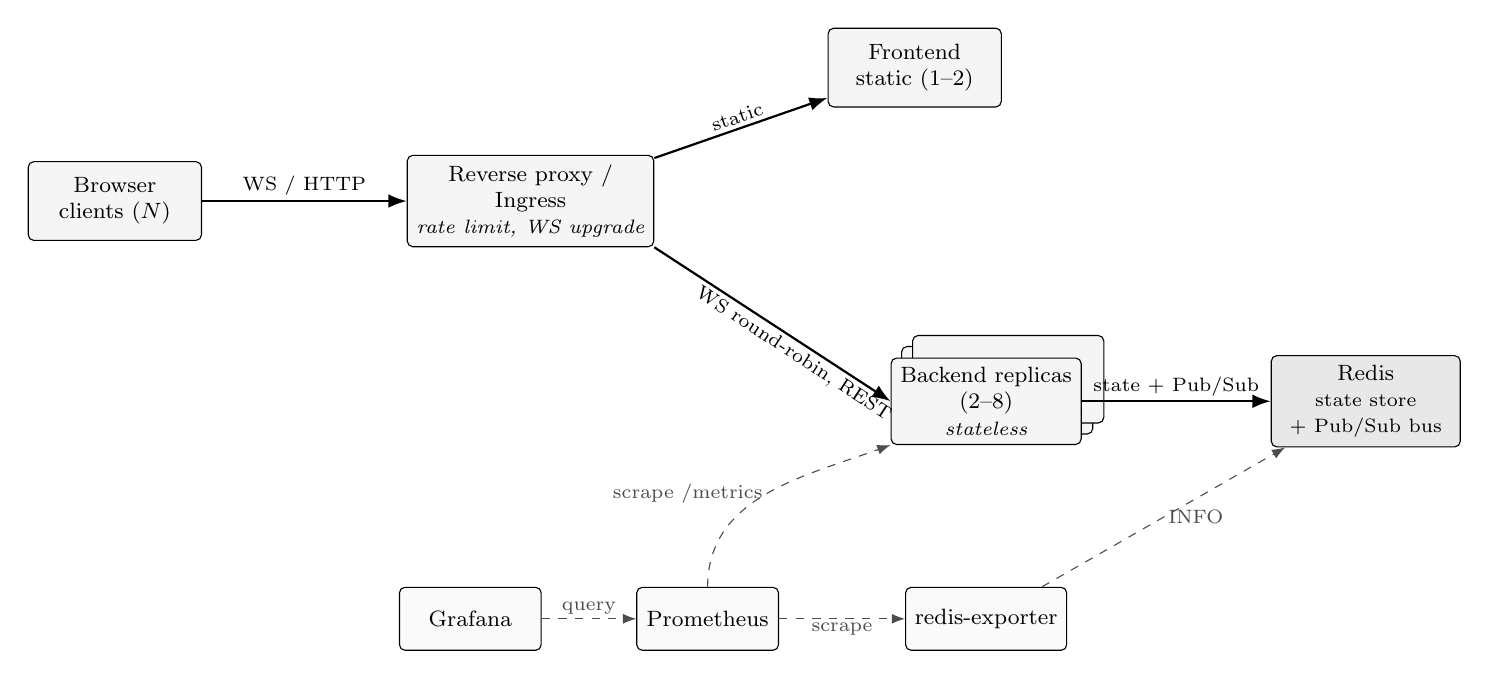
\begin{tikzpicture}[
    every node/.style={font=\footnotesize},
    comp/.style={draw, rounded corners=2pt, align=center,
                 minimum height=10mm, minimum width=22mm, fill=gray!8},
    store/.style={comp, fill=gray!18, minimum width=24mm},
    mon/.style={draw, rounded corners=2pt, align=center,
                minimum height=8mm, minimum width=18mm, fill=gray!4},
    link/.style={-Latex, thick},
    scrape/.style={-Latex, dashed, gray!60!black},
    lbl/.style={font=\scriptsize, inner sep=1.5pt},
  ]
    \node[comp] (clients) {Browser\\ clients ($N$)};
    \node[comp, right=26mm of clients] (proxy)
      {Reverse proxy /\\ Ingress\\ \scriptsize\itshape rate limit, WS upgrade};
    \node[comp, above right=6mm and 22mm of proxy] (front)
      {Frontend\\ static (1--2)};
    \node[comp, below right=14mm and 30mm of proxy] (be)
      {Backend replicas\\ (2--8)\\ \scriptsize\itshape stateless};
    % stack effect behind the backend node (suggests replication)
    \begin{scope}[on background layer]
      \draw[fill=gray!8, rounded corners=2pt]
        ([xshift=1.4mm,yshift=1.4mm]be.south west) rectangle
        ([xshift=1.4mm,yshift=1.4mm]be.north east);
      \draw[fill=gray!8, rounded corners=2pt]
        ([xshift=2.8mm,yshift=2.8mm]be.south west) rectangle
        ([xshift=2.8mm,yshift=2.8mm]be.north east);
    \end{scope}
    \node[store, right=24mm of be] (redis)
      {Redis\\ \scriptsize state store\\ \scriptsize $+$ Pub/Sub bus};
    % monitoring row
    \node[mon, below=18mm of be.south] (exp) {redis-exporter};
    \node[mon, left=16mm of exp] (prom) {Prometheus};
    \node[mon, left=12mm of prom] (graf) {Grafana};

    % data-plane edges
    \draw[link] (clients) -- node[lbl, above]{WS / HTTP} (proxy);
    \draw[link] (proxy) -- node[lbl, sloped, above]{static} (front);
    \draw[link] (proxy.south east) -- node[lbl, sloped, below, pos=0.62]{WS round-robin, REST} (be.west);
    \draw[link] (be.east) -- node[lbl, above]{state $+$ Pub/Sub} (redis);
    % monitoring (control-plane) edges
    \draw[scrape] (exp) -- node[lbl, right]{INFO} (redis);
    \draw[scrape] (prom) -- node[lbl, below]{scrape} (exp);
    \draw[scrape] (prom.north) to[out=90, in=200]
      node[lbl, left]{scrape /metrics} (be.south west);
    \draw[scrape] (graf) -- node[lbl, above]{query} (prom);
  \end{tikzpicture}%
  }
  \caption{Deployment view of the platform. Solid arrows carry the game
    data plane (client traffic, state access, the inter-replica Pub/Sub
    bus); dashed arrows are the pull-based monitoring plane. The backend
    tier is stateless and horizontally scalable (2--8 replicas), while
    Redis is a single instance playing both the authoritative state store
    and the message-broker role.}
  \label{fig:deployment}
\end{figure}

\paragraph{Network placement.}
All server-side components run in the same cluster/datacenter --- distribution
here serves fault tolerance and scalability, not geo-proximity
(\cref{ds-features}). Latency-critical hops (replica $\leftrightarrow$
store) are intra-cluster and sub-millisecond, which the design exploits
freely (several store round-trips per game action are acceptable). Clients
reach the cluster over the public Internet through the single proxy entry
point. Internally, the network is segmented into four bridge networks
(\cref{tab:networks}): the proxy can reach the frontend and the backend
pool but \emph{not} the store; the store sits on two networks, reachable by
the backends (on the data network, the latency-critical path) and by the
observability stack (on the monitoring network, so the exporter can scrape
it). The edge tier and the store therefore share no network at all, which
confines the blast radius of a compromised edge component.

\begin{table}[H]
  \centering
  \caption{Network membership of each component in the Docker Compose
    topology (the Kubernetes deployment reproduces the same segmentation
    through separate Services and namespaced routing). Two components can
    talk at the network layer \emph{iff} they share a bridge network. The
    edge proxy shares no network with the store, which is the property that
    confines the blast radius of a compromised edge; the store is reachable
    on \texttt{data\_net} by the backends and on \texttt{monitoring\_net} by
    the observability stack.}
  \label{tab:networks}
  \begin{tabular}{lcccc}
    \toprule
    & \multicolumn{4}{c}{\emph{Bridge network}} \\
    \cmidrule(l){2-5}
    Component
      & \texttt{frontend} & \texttt{backend} & \texttt{data}
      & \texttt{monitoring} \\
    \midrule
    Reverse proxy / Ingress      & $\bullet$ & $\bullet$ &           &           \\
    Frontend static server       & $\bullet$ &           &           &           \\
    Backend replica ($\times N$) &           & $\bullet$ & $\bullet$ &           \\
    Redis (store $+$ bus)        &           &           & $\bullet$ & $\bullet$ \\
    Prometheus                   &           & $\bullet$ &           & $\bullet$ \\
    Grafana                      &           &           &           & $\bullet$ \\
    redis-exporter               &           &           &           & $\bullet$ \\
    \bottomrule
  \end{tabular}
\end{table}

\paragraph{Naming and discovery.}
Components find each other by \emph{name}, never by address, at every level:

\begin{itemize}
  \item clients use one virtual host (e.g.\ \texttt{game.local}) for
  everything --- SPA, API, and real-time endpoint differ only by path, so
  the SPA needs no per-environment endpoint configuration (location
  transparency at the edge);

  \item the proxy resolves the backend pool through the platform's
  internal DNS \emph{at request time} (not at start-up), so replicas
  added or removed by scaling are picked up without reloading the proxy
  --- DNS-based service discovery;

  \item backends reach the store through a stable service name
  configured via environment (twelve-factor style), identical in every
  environment;

  \item replicas do \emph{not} discover each other at all: the
  publish/subscribe bus makes peer discovery unnecessary
  (\cref{architecture}).
\end{itemize}

\subsection{Modelling}\label{modelling}

\paragraph{Domain entities.}
The domain model is small and centred on the room:

\begin{description}
  \item[Room] an independent match container, identified by its code; it
  owns all other entities and is the unit of isolation (and of
  publish/subscribe topicality).
  \item[Player] nickname, secret \emph{role}, liveness (\emph{alive}),
  connectivity (\emph{connected}), readiness, host flag, and per-round
  action flags (\emph{has voted}, \emph{has acted}).
  \item[GameState] the room's phase (\textsc{lobby}, \textsc{day},
  \textsc{voting}, \textsc{night}, \textsc{ended}), round number, phase
  deadline (\emph{timer end}), match configuration (wolf/seer counts),
  host identity, ready set, winner, and a monotonically increasing
  \emph{state version} used to track update ordering.
  \item[Votes] two separate ballots: the public day vote (voter
  $\rightarrow$ target, including a distinguished \emph{skip} target) and
  the secret wolf vote; plus the seer's nightly inspection choice.
  \item[Chat message] sender, text, and channel; chat is transient ---
  relayed, never stored.
\end{description}

\paragraph{Mapping entities to infrastructure.}
All authoritative entity state lives in the shared store, namespaced per
room; nothing authoritative lives in a replica's memory. Clients hold only
a \emph{view}: a local copy of the last received snapshot/events used for
rendering, plus their own identity. Replicas hold only \emph{ephemeral
operational} state --- the registry of locally connected sockets and the
in-memory phase-timer tasks --- which is reconstructible and whose loss is
tolerated by design (\cref{fault-tolerance}). Chat messages are the one
entity deliberately \emph{not} stored anywhere: they are fanned out and
forgotten, since match chat has no value after the fact and persisting it
would create the only durable personal data in the system. All stored
state carries a time-to-live measured in hours, making abandoned rooms
garbage-collect themselves.

\paragraph{Domain events.}
The system is event-sourced at the \emph{interaction} level (not at the
storage level): every relevant fact is a named event. The main families
are:

\begin{itemize}
  \item \emph{room membership}: player joined, player left, host changed,
  player kicked;
  \item \emph{lobby}: settings updated, player ready changed, game start;
  \item \emph{game progression}: role assigned (private), phase changed,
  vote update, player eliminated, no elimination, player killed, seer
  result (private), game ended;
  \item \emph{synchronisation}: game state sync (the full authoritative
  snapshot);
  \item \emph{system}: chat message, error.
\end{itemize}

\paragraph{Message sorts.}
Three sorts of messages are exchanged, with different directions and
semantics:

\begin{description}
  \item[Commands] (client $\rightarrow$ server): requests to change state ---
  cast vote, wolf vote, seer action, update settings, set ready, start
  game, kick player, restart. Commands are \emph{validated} against the
  authoritative state and can be rejected (an \emph{error} event answers
  the issuer only).
  \item[Events] (server $\rightarrow$ clients, and server $\rightarrow$
  server via the bus): notifications of state changes, as listed above.
  Events sent between replicas carry an envelope with a unique event id,
  the room id, the \emph{sender replica id} (for deduplication), a
  timestamp, and optionally a \emph{target client id} marking the event
  as private unicast (delivered only to that client's socket, wherever it
  is connected).
  \item[Queries] (client $\rightarrow$ server, request/response): the
  lobby list and the health check. Queries never modify state and can be
  answered by \emph{any} replica, since all read the same store.
\end{description}

\paragraph{System state.}
Summarising, the authoritative system state comprises, per room: the room
snapshot (denormalised view for fast synchronisation of joining clients),
the game state record, the player registry, the three ballot registries,
and the phase deadline; globally, a registry of \emph{active rooms} (rooms
with a match in progress) used by the recovery sweeper, and short-lived
\emph{advancement locks} (\cref{data-and-consistency-issues}).

\subsection{Interaction}\label{interaction}

Interaction combines four patterns, each used where its coupling
characteristics fit.

\paragraph{Request/response} is used only for queries (lobby list, health
checks) and for serving static assets. It is the natural pattern for
stateless, client-initiated reads, and any replica can play the responder
role.

\paragraph{Publish/subscribe, twice.}
The core gameplay flow enacts publish/subscribe at two nested levels:

\begin{enumerate}
  \item \emph{client-facing}: joining room $R$ subscribes a client to
  $R$'s event stream over its persistent connection; the serving replica
  is the broker for its local subscribers;

  \item \emph{replica-facing}: each replica subscribes to the bus channel
  of every room for which it currently hosts at least one client
  (unsubscribing when its last local member leaves --- subscriptions track
  actual interest and cost nothing for idle rooms). Every event a replica
  produces is both emitted to its local subscribers \emph{and} published
  on the room channel.
\end{enumerate}

A replica receiving a bus message relays it to its local room members ---
unless the message's \emph{sender id} is its own, in which case it drops it:
this sender-based \textbf{deduplication} prevents the double delivery that
would otherwise occur on the originating replica (which already emitted
locally before publishing). Local emission is done \emph{before/besides}
publication on purpose: clients on the originating replica get minimal
latency, and a bus outage degrades cross-replica delivery only
(\cref{fault-tolerance}).

The typical fan-out of a game action is therefore:

\begin{enumerate}
  \item client $C_1$ (on replica $A$) sends the \emph{cast vote} command;
  \item $A$ validates it against the store, records the vote atomically,
  and builds the \emph{vote update} event;
  \item $A$ emits the event to its local members of the room and
  publishes it on the room channel;
  \item replica $B$ receives it from the bus, sees a foreign sender id,
  and relays it to its own local members --- e.g.\ client $C_2$;
  \item both $C_1$ and $C_2$ render the same vote within milliseconds.
\end{enumerate}

\begin{figure}[H]
  \centering
  \resizebox{\textwidth}{!}{%
  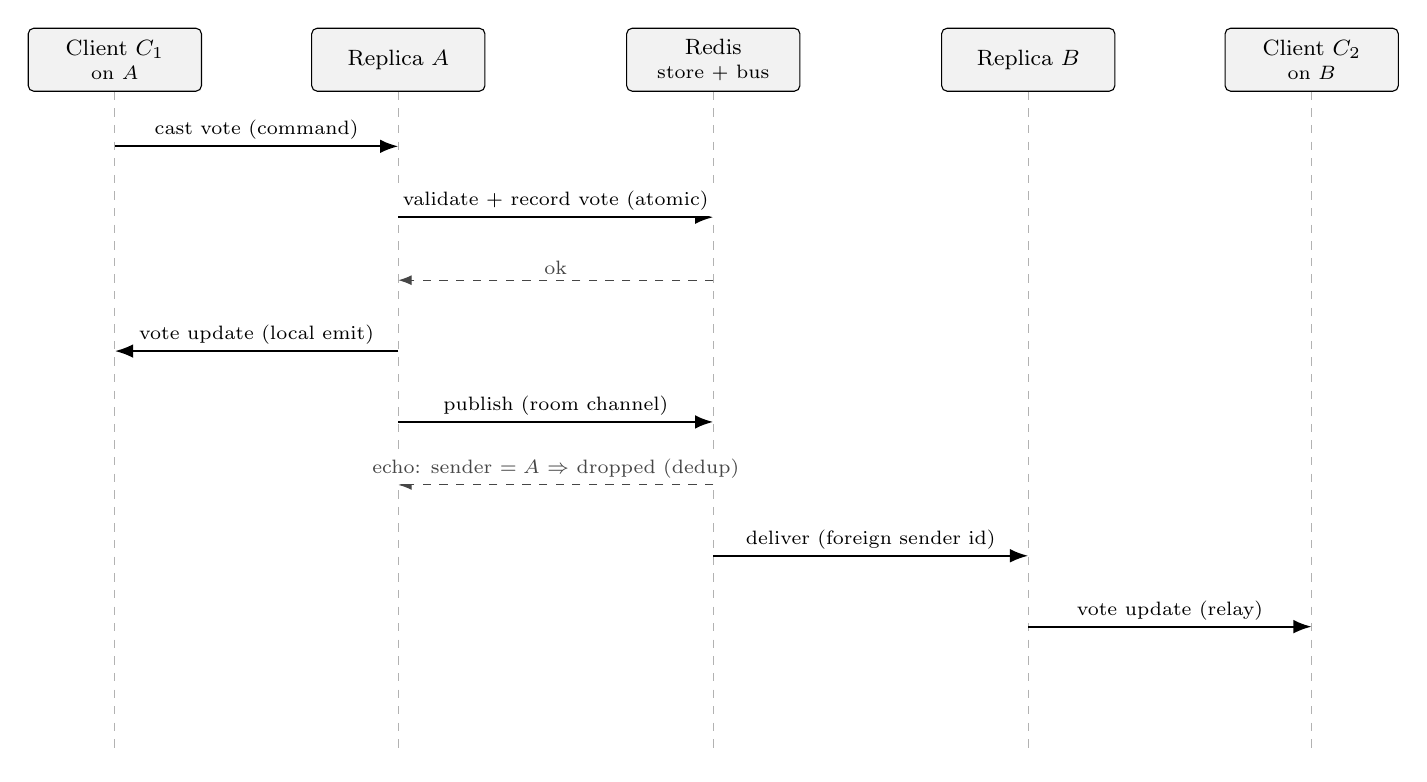
\begin{tikzpicture}[
    font=\footnotesize,
    actor/.style={draw, rounded corners=2pt, fill=gray!10,
                  minimum height=8mm, minimum width=22mm, align=center},
    msg/.style={-Latex, thick},
    ret/.style={-Latex, dashed, gray!55!black},
    lbl/.style={font=\scriptsize, inner sep=2pt, fill=white},
  ]
    % actor heads
    \node[actor] (c1) at (0,0)    {Client $C_1$\\[-1pt] \scriptsize on $A$};
    \node[actor] (a)  at (3.6,0)  {Replica $A$};
    \node[actor] (r)  at (7.6,0)  {Redis\\[-1pt] \scriptsize store $+$ bus};
    \node[actor] (b)  at (11.6,0) {Replica $B$};
    \node[actor] (c2) at (15.2,0) {Client $C_2$\\[-1pt] \scriptsize on $B$};
    % lifelines
    \foreach \n in {c1,a,r,b,c2} \draw[dashed, gray!60] (\n.south) -- ++(0,-8.4);
    % messages (time flows downward)
    \draw[msg] (0,-1.1)   -- node[lbl,above]{cast vote (command)} (3.6,-1.1);
    \draw[msg] (3.6,-2.0) -- node[lbl,above]{validate $+$ record vote (atomic)} (7.6,-2.0);
    \draw[ret] (7.6,-2.8) -- node[lbl,above]{ok} (3.6,-2.8);
    \draw[msg] (3.6,-3.7) -- node[lbl,above]{vote update (local emit)} (0,-3.7);
    \draw[msg] (3.6,-4.6) -- node[lbl,above]{publish (room channel)} (7.6,-4.6);
    \draw[ret] (7.6,-5.4) -- node[lbl,above]{echo: sender $=A$ $\Rightarrow$ dropped (dedup)} (3.6,-5.4);
    \draw[msg] (7.6,-6.3) -- node[lbl,above]{deliver (foreign sender id)} (11.6,-6.3);
    \draw[msg] (11.6,-7.2) -- node[lbl,above]{vote update (relay)} (15.2,-7.2);
  \end{tikzpicture}%
  }
  \caption{Cross-replica fan-out of a single game action (a vote). The
    originating replica $A$ writes the shared store atomically, emits to its
    own clients immediately, and publishes on the room channel; replica $B$
    relays the event to its local clients, while $A$ discards the copy the
    bus echoes back to it (sender-based deduplication). Solid arrows are
    forward messages, dashed arrows are returns.}
  \label{fig:fanout}
\end{figure}

\paragraph{Cross-replica unicast} handles \emph{private} events (role
assignment, seer result), which must reach exactly one client whose
location (which replica) the producer does not know. The event is emitted
directly if the target's socket is local, \emph{and} published with the
\emph{target client id} set: each replica receiving it delivers it only if
it currently hosts that client's socket, and never broadcasts it. This
preserves both location transparency and secrecy (FR5, FR8).

\paragraph{Periodic anti-entropy broadcast.}
Because the bus offers at-most-once delivery (\cref{fault-tolerance}), a
fourth, time-driven interaction complements the event flow: every few
seconds each replica re-derives the authoritative snapshot of its active
rooms and broadcasts it as a \emph{game state sync} event. Clients treat
snapshots as absolute truth, overwriting their local view --- so any event
missed through a lost bus message or a broken connection is repaired within
one period (NFR3). The same snapshot is sent point-to-point to every
(re)connecting client as the first message, making reconnection and initial
join the same code path (FR11).

\subsection{Behaviour}\label{behaviour}

\paragraph{The match as a replicated state machine.}
A match evolves through the phase state machine
\[
\textsc{lobby} \rightarrow \textsc{night} \rightarrow \textsc{day}
\rightarrow \textsc{voting} \rightarrow \textsc{night} \rightarrow \cdots
\rightarrow \textsc{ended} \; (\rightarrow \textsc{lobby}),
\]
where the \textsc{voting}$\to$\textsc{night} transition resolves the public
lynching, the \textsc{night}$\to$\textsc{day} transition resolves the wolf
kill and the seer inspection, every resolving transition runs the win check
(possibly short-circuiting to \textsc{ended}), and the host may loop an
ended match back to the lobby. Transitions are triggered by \emph{either}
the phase deadline expiring \emph{or} the phase completing early (all
living players have voted; all wolves and the seer have acted) \emph{or} a
decisive disconnection.

\paragraph{Backend replicas (stateless, reactive).}
Each replica is a purely reactive component: it responds to client
commands, bus messages, connection lifecycle events, and two internal
clocks. Since replicas keep no authoritative state, \emph{any} replica can
process \emph{any} trigger for \emph{any} room --- correctness is delegated
to the store's atomic operations rather than to replica identity. The two
internal clocks are:

\begin{itemize}
  \item the \emph{phase timers}: when a replica performs a phase
  transition it schedules an in-memory timer for the new deadline (the
  deadline itself --- an absolute timestamp --- is stored authoritatively).
  Timers are a local optimisation for prompt advancement, not a
  correctness mechanism: a timer firing checks the \emph{stored} deadline
  first and aborts if the phase has meanwhile advanced elsewhere
  (stale-timer guard);

  \item the \emph{sweeper}: every couple of seconds each replica scans
  the active-rooms registry for matches whose stored deadline has passed
  and advances them. This makes phase progression survive the death of
  the replica that held the in-memory timer (NFR2): the match advances
  within one sweep period, whichever replica notices first.
\end{itemize}

Both the timer path and the sweeper path (and the explicit
client-triggered advancement) funnel into a single advancement routine
guarded by a short-TTL \emph{distributed lock} acquired atomically in the
store: exactly one trigger wins per deadline, so concurrent triggers on
different replicas cannot double-advance a phase or eliminate two players
(NFR4). The lock is released explicitly once the advancement completes,
through an atomic compare-and-delete (a Lua script that removes the key only
if this replica is still its owner), so a replica can never release a
competitor's lock. Its short TTL (10\,s, far below any phase duration) is a
safety fallback: should the holder crash mid-advancement, the lock frees
itself instead of blocking the phase forever.

\paragraph{Who updates the state.}
Only backend replicas write to the store, and only in reaction to
validated commands or owned transitions; every write is atomic
(\cref{data-and-consistency-issues}). Clients never write state --- they
send commands and render events. The proxy and monitoring components are
stateless with respect to the domain.

\paragraph{Clients (stateful views).}
The client keeps a local replica of the room view and applies events
optimistically as they arrive; on any \emph{game state sync} it discards
its view and adopts the snapshot. On disconnection it re-connects with the
same identity and is treated as a rejoin: mid-game it re-receives its
secret role privately and the current snapshot; in the lobby it simply
re-enters as a new member. On the server side, a disconnection during a
match marks the player \emph{disconnected} but keeps them alive, and
\emph{pauses} the match while starting a bounded \emph{grace timer}: the
player may reconnect (to any replica, which cancels the timer --- the
expiry handler also re-checks the store's \emph{connected} flag to cover a
reconnection landing on a different replica) and resume their seat, so a
transient network drop does not cost the match. Host promotion is likewise
deferred while the grace timer is pending, so a returning host reclaims its
role. Only if the timer expires without a reconnection is the player marked
as having \emph{fled} --- treated as an elimination, to avoid stalling the
phase-completion checks --- after which the match resumes and the win check
is re-run (FR9, FR11, FR12). A player who was already eliminated (a
spectator) leaving triggers an immediate host promotion and win check
without pausing.

\subsection{Data and Consistency Issues}\label{data-and-consistency-issues}

\paragraph{What is stored, and why key--value.}
All data described in \cref{modelling} is stored in the shared in-memory
store as JSON-serialised values under a per-room key namespace: a string
key per room snapshot and per game-state record, hash structures for the
player registry and the ballots (field = player id), a string for the
phase deadline, and a set for the active-rooms registry. A key--value/hash
model fits naturally: the data is small, schema-light, always accessed by
known key (room id, player id), and never queried relationally --- there are
no joins, no secondary indexes, no cross-room queries except the lobby
list, which is served by an incremental scan of the room-snapshot
namespace. A relational or document database would add operational weight
(IR3) and millisecond-scale latency to a path that is hit several times
per game action. Durability requirements are also modest (game state is
ephemeral, \cref{ds-features}), so an in-memory store with lightweight
disk persistence (periodic snapshots plus an append-only log fsynced every
second) is an appropriate trade-off: after a store crash, at most the last
second of updates is lost --- for a game this means, at worst, re-casting a
vote.

\paragraph{Who reads and writes.}
Only backend replicas access the store. Reads happen on every command
validation, on every client (re)connection (snapshot), on the periodic
sweeper and anti-entropy scans, and on lobby-list queries. Writes happen
on membership changes, lobby reconfiguration, votes and night actions, and
phase transitions. Reads and writes are heavily concurrent: the same
room's state is routinely accessed by several replicas at once (their
clients act simultaneously), which is precisely where the consistency
issues below arise.

\paragraph{Consistency strategy: strong at the store, eventual at the clients.}
The design splits the consistency question in two:

\begin{itemize}
  \item \textbf{Authoritative state} must never violate the game
  invariants (NFR4). All multi-step updates are made \emph{atomic at the
  store}, which acts as the single serialisation point (an atomic data
  object): every replica's writes are applied in a single total order, so
  the stored state is sequentially consistent and lost updates are
  prevented by construction rather than by inter-replica coordination.
  Four mechanisms are used, in increasing strength:
  %
  \begin{enumerate}
    \item \emph{single-operation atomicity} for naturally atomic updates
    (a vote is one hash-field write);
    \item \emph{atomic create-if-absent} for the room bootstrap: when two
    strangers create the same room simultaneously on different replicas,
    only one initial-state write succeeds, and its author becomes host ---
    eliminating the ``double host'' race (FR1);
    \item \emph{optimistic transactions} (watch--modify--retry) for
    read-modify-write patches of the game-state record: a concurrent
    modification aborts and retries the patch instead of silently
    overwriting it (e.g.\ a settings update racing a ready toggle). Each
    successful patch also increments the record's \emph{state version};
    \item \emph{mutual exclusion} where an entire multi-key procedure
    must run at most once per deadline: phase advancement takes the
    atomic short-TTL lock described in \cref{behaviour}.
  \end{enumerate}

  \item \textbf{Client views} are only \emph{eventually
  consistent}~\cite{vogels2009eventually}: an event can reach the clients
  of different replicas at slightly different times, or be missed
  entirely (at-most-once bus). The design accepts this --- sub-second
  divergence of rendered views is imperceptible in a chat-paced game ---
  and guarantees \emph{convergence} instead: the periodic anti-entropy
  snapshot (\cref{interaction}) overwrites any diverged view within
  seconds (NFR3). Snapshots are recomputed from authoritative state, so
  convergence is toward the correct value, not merely toward agreement.
\end{itemize}

This split is the project's answer to the CAP
trade-off~\cite{gilbert2002brewer}: rather than paying for consensus among
replicas~\cite{fischer1985impossibility}, the design concentrates
consistency in one store and treats replicas as stateless caches of
nothing --- they hold no divergable copy of domain state at all.

\paragraph{Shared data between components.}
Beyond domain state, replicas share only two coordination artefacts, both
in the store: the active-rooms set (work list for sweeper/anti-entropy)
and the advancement locks. Notably, replicas do \emph{not} share their
connection registries: which client is connected to which replica is
deliberately kept local, and cross-replica delivery is solved by
publish/subscribe semantics instead of by a shared session directory ---
one less piece of shared mutable state to keep consistent.

\subsection{Fault-Tolerance}\label{fault-tolerance}

The failure model is crash (fail-stop) of any single server-side process,
plus message loss: the inter-replica bus provides \emph{at-most-once}
delivery (a publish reaching a momentarily disconnected subscriber is
simply gone), and the network is assumed unreliable in all the classic
ways~\cite{rotem2006fallacies}.

\paragraph{Replication and redundancy.}
The \emph{service} is actively replicated ($\geq 2$ identical replicas,
active--active): any replica serves any room, so a crash removes capacity
but no function. \emph{Data} is not replicated across nodes (single
store); it is instead made recoverable by the store's own disk persistence
(snapshot + append-only log), which restores state on restart with at most
one second of loss. This asymmetry is deliberate: replicating the service
is cheap (it is stateless), replicating the store safely is not (it needs
primary election and failover protocols), and the dependability
requirement --- do not lose running matches --- is met already if the store's
downtime is short, because all other components mask it (below).

\paragraph{Heart-beating, timeouts, retries.}
Failure detection is timeout-based at every seam of the system:

\begin{itemize}
  \item \emph{orchestrator} $\to$ \emph{replicas}: periodic liveness
  probes restart a wedged replica; readiness probes remove a replica from
  load balancing until it is actually able to serve (connected to the
  store), so clients are never routed to a half-alive instance;
  \item \emph{clients} $\leftrightarrow$ \emph{replicas}: the realtime
  protocol exchanges application-level heartbeats; a client detecting a
  dead connection reconnects automatically (through the balancer, hence
  possibly to a \emph{different} replica) and is re-synced by snapshot;
  \item \emph{replicas} $\to$ \emph{store}: every publish is retried a
  bounded number of times with exponential back-off before being declared
  lost; the bus \emph{listener} detects connection failure and enters an
  unbounded reconnect loop with capped exponential back-off,
  re-subscribing all its channels once the store returns --- without this,
  a store blip would silently and permanently cut a replica off the bus;
  \item \emph{proxy} $\to$ \emph{replicas}: connect/read timeouts plus
  request-time DNS re-resolution route around dead replicas.
\end{itemize}

\paragraph{What happens when each component fails.}

\begin{description}
  \item[A backend replica crashes.] Its clients' connections drop; they
  reconnect through the balancer to surviving replicas and receive the
  authoritative snapshot --- nothing is lost because the replica held
  nothing authoritative. Its in-memory phase timers die with it: the
  cross-replica \emph{sweeper} (\cref{behaviour}) notices the expired
  stored deadline within a couple of seconds and advances the match on
  another replica, under the advancement lock. This is the scenario of
  NFR2 and is exercised directly by the validation suite
  (\cref{automatic-testing}).

  \item[The store becomes unreachable.] Commands requiring state fail
  cleanly (clients get error events and can retry); already-delivered
  views remain rendered, so ongoing discussion is not interrupted. Each
  replica's listener keeps retrying; on recovery, publishes resume,
  channels are re-subscribed, and the next anti-entropy round re-syncs
  every client. Events lost on the bus during the outage are repaired by
  the same anti-entropy mechanism --- the design never assumes bus
  reliability, only store reliability \emph{over time}.

  \item[The proxy or frontend crashes.] Both are stateless; the
  orchestrator restarts them, and clients experience a transient
  connection error. The monitoring stack is entirely out of the game's
  fault path: its failure affects observability only.
\end{description}

\begin{table}[H]
  \centering
  \footnotesize
  \setlength{\tabcolsep}{6pt}
  \renewcommand{\arraystretch}{1.3}
  \caption{Failure modes and how the platform tolerates them. Detection is
    timeout-based at every seam; recovery never depends on the failed
    component itself, and the fault of any single server-side component
    leaves running matches intact.}
  \label{tab:failure-modes}
  \begin{tabular}{@{}
    >{\raggedright\arraybackslash}p{2.4cm}
    >{\raggedright\arraybackslash}p{3.1cm}
    >{\raggedright\arraybackslash}p{4.8cm}
    >{\raggedright\arraybackslash}p{2.6cm}@{}}
    \toprule
    \textbf{Failure} & \textbf{Detected by} & \textbf{Recovery}
      & \textbf{Player impact} \\
    \midrule
    Backend replica crash
      & orchestrator liveness/readiness probes; client heartbeat
      & clients reconnect through the balancer to a surviving replica and
        re-sync by snapshot; the sweeper advances the phase timer under the
        advancement lock
      & brief reconnect; match continues (NFR2) \\
    Store (Redis) unreachable
      & Pub/Sub listener error; failed store commands
      & listener reconnect loop with back-off $+$ channel re-subscription;
        publish retries; anti-entropy re-syncs every client on recovery
      & state-changing commands rejected briefly; rendered views persist \\
    Proxy / frontend crash
      & orchestrator liveness probe
      & stateless restart; request-time DNS re-resolution routes around it
      & transient connection error, auto-reconnect \\
    Client disconnect / network drop
      & socket close $+$ missed heartbeats
      & match paused, grace timer started; reconnect (to any replica)
        resumes it, otherwise the player is dropped
      & short pause; resumes on return \\
    Monitoring stack down
      & Prometheus self-monitoring / alerts
      & stateless restart
      & none (observability only) \\
    \bottomrule
  \end{tabular}
\end{table}

\paragraph{Error handling within the protocol.}
Invalid or unauthorised commands (wrong phase, non-host configuration
attempt, dead voter\ldots) are rejected by validation against
authoritative state and answered with a private \emph{error} event ---
misbehaving or buggy clients cannot corrupt state, only annoy themselves.
Unexpected exceptions in event handlers are caught per-event: one
malformed message cannot take down a replica's event loop. Corrupted
records read from the store (failed deserialisation) are logged and
skipped rather than crashing the reader.

\subsection{Availability}\label{availability}

\paragraph{Caching.}
There is no cache tier, by design: the ``database'' is itself an in-memory
store with sub-millisecond access, so a cache in front of it would add a
consistency problem without a latency benefit. Two cache-like mechanisms
exist nonetheless: the per-room \emph{snapshot} record is a denormalised,
ready-to-send view maintained alongside the normalised state (a
materialised view, refreshed on every relevant change and by anti-entropy),
so that the hot path of client synchronisation is one read; and each
\emph{client} caches the room view locally between events, which is what
keeps the UI responsive and readable even during a brief server-side
outage. Static SPA assets are served with standard HTTP caching.

\paragraph{Load balancing.}
Load balancing happens at connection granularity at the entry proxy:
new realtime connections are assigned to backend replicas
\emph{round-robin}. Round-robin is the right policy for long-lived
connections: each connection is a lasting resource commitment, so the goal
is to spread \emph{connection counts} evenly. Latency-aware policies were
evaluated and rejected because a persistent connection produces no
response-time signal until it closes --- such policies degenerate to piling
every connection onto one replica. Because clients reconnect through the
balancer, load also \emph{re}-balances naturally after failures and
scale-ups. Horizontal elasticity complements balancing: replicas are
scaled automatically between a floor of 2 (fault tolerance) and a ceiling
of 8, scaling up aggressively on load spikes and down slowly --- draining a
replica disconnects its clients, so scale-down is deliberately damped to
once a minute after a 5-minute stabilisation window (NFR5, NFR8).
%
The ceiling of 8 is a pragmatic cap rather than a hard technical limit of
the stateless tier: past a certain point the real bottleneck becomes the
single Redis instance, which every replica shares as both state store and
message bus, so adding backends only shifts pressure onto it instead of
increasing capacity. Eight replicas --- at the roughly 80 concurrent
WebSocket connections per replica used to size the connection-based scaling
metric, some \(640\) simultaneous players --- comfortably exceed the load a
casual party game must sustain, while keeping the whole platform within the
single-machine, zero-budget deployment target (minikube, IR3). Lifting the
ceiling meaningfully would first require making the store
highly available (\cref{future-works}).

\paragraph{Behaviour under network partition.}
Applying CAP~\cite{gilbert2002brewer} per partition scenario:

\begin{description}
  \item[Client partitioned from the cluster.] The match goes on: phases
  advance server-side regardless of individual clients (timers are
  authoritative), and the partitioned player's inaction is handled by the
  same rules as any inaction; on prolonged disconnection during a match
  the player is marked as having fled. On heal, the client re-syncs by
  snapshot. This favours availability for the \emph{group} over the
  individual --- the correct choice for a party game, where one player's
  bad network must not stall everyone.

  \item[Replica partitioned from the store.] The replica keeps its
  clients connected but refuses state-changing commands (it cannot
  validate them): it degrades to read-only availability on stale views
  rather than guessing --- for authoritative writes the design chooses
  consistency over availability, because a wrong elimination is worse
  than a delayed one. Meanwhile its readiness probe fails, so the
  balancer stops routing \emph{new} connections to it.

  \item[Split between replicas (bus unreachable, store reachable).]
  Impossible to sustain silently in this topology --- bus and store are the
  same component --- but the at-most-once analysis of
  \cref{fault-tolerance} covers transient versions of it: views diverge
  for at most one anti-entropy period, then converge. Writes remain
  correct throughout, since they serialise at the store.
\end{description}

\subsection{Security}\label{security}

\paragraph{Authentication.}
There is no account system: players self-identify with a nickname scoped
to a room, which doubles as their client identifier. This is a conscious
trade-off (\cref{ds-features}): the product is a casual party game among
acquaintances, no sensitive data is at stake, and login friction would
hurt the primary use case more than impersonation would. The nickname is,
however, weakly protected where it matters for gameplay: a name already
connected to a room cannot be taken by a second connection (preventing
casual impersonation and accidental double tabs, FR14), and the same
identity is what lets a disconnected player resume their seat (FR11).

\paragraph{Authorization.}
Access control is enforced \emph{server-side on every command}, on the
authoritative state --- never on client claims. It is a small role-based
scheme with three axes:

\begin{itemize}
  \item \emph{platform role}: host-only rights (configure the match,
  start it, kick, restart) are checked against the stored host identity;
  \item \emph{game role and liveness}: only living players may vote; only
  wolves may wolf-vote; only the seer may inspect; spectators
  (eliminated players) retain read access only;
  \item \emph{phase}: every command is valid only in its phase
  (configuration in \textsc{lobby}, votes in \textsc{voting}, night
  actions in \textsc{night}), which blocks whole classes of
  out-of-order exploits.
\end{itemize}

Information-flow control complements access control: secret data (roles,
wolf ballots, seer results) is delivered only over private unicast events
and is systematically excluded from broadcast snapshots until game end ---
so even a modified client observing all its traffic learns nothing it
should not know (FR5, FR8). Room joining is likewise gated: matches in
progress refuse strangers (FR14).

\paragraph{Perimeter and cryptography.}
The proxy is the only exposed component; internal components are on
segregated networks and unreachable from outside
(\cref{infrastructure}). It applies per-IP rate limits (separate budgets
for API calls and connection attempts) to blunt abuse and trivial
denial-of-service, sets standard security headers, and hides
implementation details. No custom cryptographic schema is used ---
there are no passwords or tokens to protect, and transport encryption
(TLS) is a deployment concern the proxy is already prepared for
(certificates would be terminated there in a public deployment; the local
course deployments run plain HTTP). Interactive API documentation is
disabled outside development.

\section{Implementation}\label{implementation}

This section binds the design of \cref{design} to concrete technologies,
motivating each choice.

\paragraph{Network protocols.}
Client--server realtime communication uses
\textbf{Socket.IO}~\cite{socketio} on top of WebSocket (over TCP/HTTP),
with automatic fallback to HTTP long-polling. Socket.IO was preferred to
raw WebSocket because it provides, out of the box, exactly the machinery
the design requires: named events, \emph{rooms} (the per-room topic
abstraction of \cref{interaction}), application-level heartbeats
(ping/pong) for failure detection, and automatic client reconnection with
back-off --- re-implementing these reliably over raw WebSocket is
error-prone and out of scope. Queries (lobby list, health) use plain
\textbf{HTTP/1.1} REST endpoints. Inter-replica communication uses the
\textbf{Redis serialization protocol (RESP)}, both for data operations and
for Pub/Sub~\cite{redis}. All traffic from clients enters through a single
HTTP origin; the proxy upgrades WebSocket connections
(\texttt{Upgrade}/\texttt{Connection} headers) and keeps them alive with
hour-long read timeouts.

\paragraph{In-transit data representation.}
All payloads --- client events, bus messages, stored values --- are
\textbf{JSON}. The dominant consumer is a browser, so JSON is the
zero-friction choice; payloads are small (well under the enforced 1\,MB
cap), so a binary format (e.g.\ Protocol Buffers) would buy little except
schema tooling. Message \emph{schemas} are nonetheless explicit in code:
every event family has a typed model --- Pydantic models for the
\texttt{RedisEvent} bus envelope (event id, type, room, sender replica,
timestamp, payload, optional target client) and the \texttt{WSMessage}
client envelope, plus dataclasses per event payload --- so malformed
messages are rejected at the boundary by validation rather than deep in
game logic.

\paragraph{Database access.}
The store is \textbf{Redis 7}~\cite{redis}, accessed through its native
asynchronous Python client (\texttt{redis.asyncio}) --- no ORM, since the
data model is key--value by design (\cref{data-and-consistency-issues}).
The consistency mechanisms map to Redis primitives one-to-one: atomic
creation is \texttt{SET NX EX}; optimistic transactions are
\texttt{WATCH}/\texttt{MULTI}/\texttt{EXEC} with retry on
\texttt{WatchError}; the advancement lock is \texttt{SET NX} with a 10\,s
TTL; bulk player updates use pipelines (one round-trip instead of $O(n)$);
the lobby list uses cursor-based \texttt{SCAN} rather than the blocking
\texttt{KEYS}; TTLs (\texttt{SETEX}/\texttt{EXPIRE}, 6\,h, renewed on
write) garbage-collect abandoned rooms. Pub/Sub channels are named
\texttt{game:\{room\_id\}} plus one global channel.

\paragraph{Authentication and authorization.}
As designed in \cref{security}: no OAuth/JWT machinery --- identity is the
per-room nickname, transmitted in the Socket.IO handshake (auth payload or
query string) and bound server-side to the socket id by the connection
manager. Authorization is implemented as guard clauses at the top of every
command handler, reading the authoritative Redis state (host id, phase,
role, liveness) and raising domain errors that reach the offending client
as private \emph{error} events. RBAC frameworks would be
over-engineering for three roles and a dozen rules.

\subsection{Technological details}\label{technological-details}

\paragraph{Backend: Python 3.12, FastAPI, python-socketio, Uvicorn.}
The backend is an ASGI application composed of
\textbf{FastAPI}~\cite{fastapi} (REST endpoints, dependency-injected
settings via \texttt{pydantic-settings}, automatic OpenAPI docs in
development) and \textbf{python-socketio}'s \texttt{AsyncServer} mounted
on the same server, run by \textbf{Uvicorn} with the \texttt{uvloop} event
loop. An asynchronous single-threaded runtime is the natural match for
the workload identified in \cref{ds-features}: thousands of mostly idle
sockets multiplexed over one event loop, with I/O-bound handlers awaiting
Redis. Each container deliberately runs \emph{one} Uvicorn worker ---
scaling is horizontal at the container level (\cref{deployment}), which
keeps the per-process state (connection registry, timers) trivially
consistent and lets the orchestrator, not the process manager, own
scaling. Long-running concerns (Pub/Sub listener, timer sweeper,
anti-entropy) are \texttt{asyncio} background tasks started in FastAPI's
lifespan hook. Each replica identifies itself with an
\texttt{INSTANCE\_ID} taken from the \texttt{HOSTNAME} environment
variable (the pod/container name), which implements the sender-id
deduplication and lock ownership of \cref{design} with zero
configuration.

\paragraph{Frontend: Vue 3, Pinia, Vite, socket.io-client.}
The SPA uses \textbf{Vue~3} with \textbf{Pinia} stores mirroring the
domain (lobby, game, chat) and \textbf{vue-router} for the four views
(home, lobby, game, results); it is built with \textbf{Vite} and served as
static files by a minimal NGINX container. The backend origin is not
baked in at build time: a \texttt{config.js} is generated \emph{at
container start} by an entrypoint script (\texttt{envsubst} on a
template, reading the \texttt{WS\_URL} environment variable, defaulting to
same-origin), so the very same image runs under \texttt{localhost},
\texttt{game.local}, or any production domain --- an application of the
build-once/configure-at-runtime principle that keeps images
environment-agnostic.

\paragraph{Containerisation.}
Both images are multi-stage builds: the backend separates a
dependency-compilation stage from a slim runtime
(\texttt{python:3.12-slim}); the frontend builds with
\texttt{node:20-alpine} and ships only compiled assets on
\texttt{nginx:1.25-alpine}. Both run as non-root users and embed
container-level health checks. This yields small, reproducible,
least-privilege images --- the unit of deployment everywhere from Compose
to Kubernetes.

\paragraph{Edge and observability stack.}
The reverse proxy is \textbf{NGINX 1.25} (Compose) and the
\textbf{NGINX Ingress Controller} (Kubernetes), configured as per
\cref{infrastructure,availability}. Metrics use
\texttt{prometheus-fastapi-instrumentator} for HTTP metrics plus custom
counters/histograms (\cref{tab:metrics}: active connections, messages
sent/received by type, broadcast latency, Pub/Sub
publishes/failures/deduplications/reconnects),
all labelled by \texttt{instance\_id}; \textbf{Prometheus}~\cite{prometheus}
scrapes replicas and a \texttt{redis\_exporter}, evaluates recording/alert
rules (backend down, Redis down, error rates), and \textbf{Grafana} ships
with a provisioned dashboard --- so observability (NFR7) works out of the
box in both deployments.

\begin{table}[H]
  \centering
  \footnotesize
  \setlength{\tabcolsep}{6pt}
  \renewcommand{\arraystretch}{1.25}
  \caption{Custom application metrics exported on \texttt{/metrics}
    (standard HTTP metrics are added automatically by the instrumentator).
    Every metric additionally carries an \texttt{instance\_id} label, so all
    quantities can be broken down per replica; the \emph{Labels} column
    lists only the further dimensions.}
  \label{tab:metrics}
  \begin{tabular}{@{}
    >{\raggedright\arraybackslash}p{5.0cm}
    >{\raggedright\arraybackslash}p{1.6cm}
    >{\raggedright\arraybackslash}p{1.9cm}
    >{\raggedright\arraybackslash}p{4.0cm}@{}}
    \toprule
    \textbf{Metric} & \textbf{Type} & \textbf{Labels} & \textbf{Measures} \\
    \midrule
    \multicolumn{4}{@{}l}{\emph{WebSocket connections}} \\
    \texttt{ws\_active\_connections}    & Gauge   & ---        & live WS connections on the replica \\
    \texttt{ws\_connections\_total}     & Counter & ---        & connections accepted since start \\
    \texttt{ws\_disconnections\_total}  & Counter & \texttt{reason} & disconnections (normal / timeout / error) \\
    \addlinespace
    \multicolumn{4}{@{}l}{\emph{WebSocket messages}} \\
    \texttt{ws\_messages\_received\_total} & Counter & \texttt{event\_type} & client\,$\to$\,server messages, by event \\
    \texttt{ws\_messages\_sent\_total}     & Counter & \texttt{event\_type} & server\,$\to$\,client messages, by event \\
    \texttt{ws\_message\_size\_bytes}      & Histogram & ---      & size of received messages (bytes) \\
    \addlinespace
    \multicolumn{4}{@{}l}{\emph{Redis Pub/Sub bus}} \\
    \texttt{redis\_messages\_published\_total}    & Counter & \texttt{channel} & events published on the bus \\
    \texttt{redis\_messages\_received\_total}     & Counter & \texttt{channel} & events received from the bus \\
    \texttt{redis\_messages\_deduplicated\_total} & Counter & ---     & own-echo events dropped (dedup) \\
    \texttt{redis\_publish\_failures\_total}      & Counter & ---     & publishes lost after all retries \\
    \texttt{redis\_reconnects\_total}             & Counter & ---     & listener reconnects to the store \\
    \addlinespace
    \multicolumn{4}{@{}l}{\emph{Rooms \& players}} \\
    \texttt{game\_active\_rooms}   & Gauge & --- & rooms with $\geq 1$ local client \\
    \texttt{game\_active\_players} & Gauge & --- & connected players on the replica \\
    \addlinespace
    \multicolumn{4}{@{}l}{\emph{Internal latency}} \\
    \texttt{redis\_publish\_duration\_seconds} & Histogram & --- & \texttt{PUBLISH} latency to the broker \\
    \texttt{ws\_broadcast\_duration\_seconds}  & Histogram & --- & time to broadcast to a room \\
    \bottomrule
  \end{tabular}
\end{table}

\section{Validation}\label{validation}

\subsection{Automatic Testing}\label{automatic-testing}

Testing is organised in three rings, from pure logic to the deployed
system.

\paragraph{Ring 1 --- unit tests (backend and frontend).}
The backend game and lobby logic is unit-tested with \texttt{pytest} +
\texttt{pytest-asyncio} (run with \texttt{pytest} from \texttt{backend/}).
Redis is replaced by \texttt{fakeredis}, an in-process emulator honouring
the same command semantics: tests exercise the \emph{real} data-access
code, including transactions, without any running infrastructure --- fast
and CI-friendly. The suites cover role assignment and its validation
bounds (FR3, FR5), phase transitions and their resolutions --- vote
tallying with ties and skips, night kills, seer inspection, win detection
(FR6--FR9) --- host promotion on disconnect (FR12), lobby snapshot/role
visibility rules (FR5), and the state store itself. The frontend mirrors
this with \texttt{vitest} suites (run with \texttt{npm test}) for the
Pinia stores (lobby, game, chat), the socket event handling
(\texttt{gameStore.socket}), the countdown composable, and routing ---
i.e.\ the client-side reducers that turn server events into rendered
state.

\paragraph{Ring 2 --- distributed-safety tests.}
A dedicated suite (\texttt{tests/test\_distributed\_safety.py},
\texttt{pytest}) verifies the concurrency mechanisms of
\cref{data-and-consistency-issues} in isolation, one guarantee per test:
atomic room creation elects exactly one host under a simulated
double-join (FR1, NFR4); the advancement lock admits a single winner per
room while remaining independent across rooms (NFR4); optimistic patches
merge concurrent field updates and bump the version monotonically ---
i.e.\ no lost updates (NFR4); the active-rooms registry behaves as the
sweeper expects (NFR2); bulk persistence preserves per-player data.
These tests exist because such properties are exactly the ones that
manual testing cannot reliably exercise: they encode the race conditions
as deterministic scenarios.

\paragraph{Ring 3 --- end-to-end tests against the deployed system.}
Deployment automation (\cref{deployment}) makes it cheap to bring up a
production-like environment (Compose with two backend replicas, or the
Kubernetes cluster), against which three scripted Socket.IO clients
suites run (plain Python scripts under \texttt{tests/}, using the same
\texttt{socket.io} client as the real frontend):

\begin{itemize}
  \item \texttt{test\_multi\_instance.py} validates replication
  transparency (NFR1, FR10): events published by a client on replica $A$
  reach clients on replica $B$ and vice versa, local broadcast still
  works, and the sender never receives its own event twice
  (deduplication). It can target the load-balanced entry point or two
  specific pods via port-forward, asserting on the \texttt{instance\_id}
  carried by every message.

  \item \texttt{test\_reconnection.py} validates state synchronisation
  (FR11, NFR3): a fresh room yields no spurious snapshot; a client
  reconnecting to the same or to a \emph{different} replica receives the
  state produced while it was away; two clients on different replicas
  observe consistent state and player registries after churn.

  \item \texttt{load\_test.py} validates NFR5/NFR6: a multi-process
  Socket.IO load generator (hundreds of concurrent clients spread over
  several OS processes, so that the bottleneck under test is the
  platform, not the generator's event loop) measures connection success
  and event delivery under load, and is used to observe HPA scale-up and
  connection spreading live (via \texttt{kubectl get hpa -w} and the
  Grafana dashboard). A companion diagnostic script
  (\texttt{diag\_loss.py}) distinguishes real event loss from test
  artefacts.
\end{itemize}

Corner cases are covered where they live: crash-recovery of phase timers
is exercised by killing a backend pod during a scripted match (the
sweeper advances the phase within its period --- NFR2); invalid commands
(non-host configuration, dead voters, wrong-phase actions) are asserted
to produce rejections in ring-1 tests (FR3, FR7, FR14).

\subsection{Acceptance test}\label{acceptance-test}

Manual play-testing sessions were run on the full deployment (several
browsers, including different machines, behind the load balancer) for the
properties that resist automation:

\begin{itemize}
  \item \emph{perceived experience}: UI readability, timer smoothness,
  the simultaneity of phase changes and eliminations across screens ---
  qualitative judgements a script cannot make;
  \item \emph{full-game flows}: complete matches with 5+ players
  including seer play, skip votes, mid-game abandonments, kicks,
  end-game screens, and play-again loops (FR4--FR9, FR13) --- automating a
  whole match with hidden-role coordination across many scripted clients
  was judged poor value for the project scope, since the underlying
  rules are already unit-tested;
  \item \emph{operational drills}: killing pods mid-match, restarting
  Redis, and watching the system converge --- semi-automated (deployment
  scripts + dashboards) but validated by human observation of the
  resulting gameplay.
\end{itemize}

Each acceptance session mapped observed behaviour back to the acceptance
criteria of \cref{requirements}; all functional requirements were
verified on the Kubernetes deployment before delivery.

\section{Deployment}\label{deployment}

The platform supports three deployment profiles, all driven by files
versioned in the repository; complete step-by-step instructions live in
the repository \texttt{README}. \Cref{tab:profiles} summarises them.

\begin{table}[H]
  \centering
  \footnotesize
  \setlength{\tabcolsep}{6pt}
  \renewcommand{\arraystretch}{1.25}
  \caption{The three deployment profiles. They share the same images and
    configuration mechanism (\cref{technological-details}); they differ in
    what is containerised and in the target environment.}
  \label{tab:profiles}
  \begin{tabular}{@{}
    >{\raggedright\arraybackslash}p{2.6cm}
    >{\raggedright\arraybackslash}p{4.2cm}
    >{\raggedright\arraybackslash}p{3.8cm}
    >{\raggedright\arraybackslash}p{2.6cm}@{}}
    \toprule
    \textbf{Profile} & \textbf{Bring-up command} & \textbf{Brings up}
      & \textbf{Entry point} \\
    \midrule
    \textbf{1 --- Development} \newline \emph{support only, hot-reload}
      & \texttt{docker compose -f} \texttt{docker-compose-dev.yml up -d}
        \newline $+$ native \texttt{uvicorn --reload} and \texttt{npm run dev}
      & Redis, exporter, Prometheus, Grafana (backend and frontend run
        natively)
      & Vite dev server on \texttt{localhost} \\
    \addlinespace
    \textbf{2 --- Full Compose} \newline \emph{single machine, full stack}
      & \texttt{docker compose up -d} \texttt{-{}-scale backend=2}
      & NGINX, $N$ backend replicas, frontend, Redis, monitoring stack
      & \texttt{http://localhost} \\
    \addlinespace
    \textbf{3 --- Kubernetes} \newline \emph{cluster, production-like}
      & \texttt{k8s/deploy.sh} \newline (or the documented
        \texttt{kubectl apply} sequence)
      & namespace, ConfigMap/Secret, Redis $+$ PVC, backend $+$ HPA (2--8),
        frontend, monitoring, Ingress
      & \texttt{http://game.local} \newline (via \texttt{minikube tunnel}) \\
    \bottomrule
  \end{tabular}
\end{table}

\subsection{Prerequisites and configuration}

The only host requirements are Docker Desktop 24+ with Compose v2 and,
for the cluster profile, \texttt{kubectl} 1.28+ and \texttt{minikube}
1.32+ (with the \texttt{ingress} and \texttt{metrics-server} addons).
All application configuration flows through \emph{environment variables}
with sensible defaults (Redis URL, channel prefix, phase durations, log
level): locally a \texttt{backend/.env} is created from the provided
\texttt{.env.example}; in Compose the variables are set on the service;
in Kubernetes they come from a \texttt{ConfigMap} (non-sensitive values)
with a \texttt{Secret} template for credentials. No file needs editing to
switch environments --- the same images run everywhere
(\cref{technological-details}).

\subsection{Profile 1 --- development (support services only)}

\texttt{docker compose -f docker-compose-dev.yml up -d} starts only the
stateful/support services (Redis, its exporter, Prometheus, Grafana) on a
dedicated network and volumes, while backend
(\texttt{uvicorn main:app --reload}) and frontend
(\texttt{npm run dev}) run natively with hot-reload. This keeps the edit
cycle at IDE speed while developing against real infrastructure.

\subsection{Profile 2 --- full Docker Compose}

\texttt{docker compose up -d --scale backend=2} builds and starts the
entire platform on one machine: NGINX (the only published entry point, port
80), $N$ backend replicas, the frontend, Redis, and the monitoring stack.
The Compose file encodes the design decisions of \cref{infrastructure}
directly:

\begin{itemize}
  \item \emph{four segregated bridge networks} (proxy--frontend,
  proxy--backend, backend--Redis, monitoring), so each container sees only
  what it needs;
  \item \emph{named volumes} for Redis, Prometheus, and Grafana data,
  surviving container recreation;
  \item \emph{health checks on every service} and
  \texttt{depends\_on: condition: service\_healthy}, so backends start
  only after Redis answers \texttt{PING};
  \item \emph{replica-friendly backend definition}: no fixed container
  name or published port (NGINX resolves the service name at request
  time), so \texttt{--scale backend=$N$} just works;
  \item \emph{resource limits} on the backend mirroring the Kubernetes
  requests/limits, keeping the two environments comparable.
\end{itemize}

Expected outcome: \texttt{docker compose ps} shows every service
\emph{healthy}; the game answers at \texttt{http://localhost},
Prometheus at \texttt{:9090}, Grafana at \texttt{:3001}; and
\texttt{curl http://localhost/health} returns each replica's id in
round-robin.

\subsection{Profile 3 --- Kubernetes (minikube)}

Images are built into minikube's Docker daemon, then either the
\texttt{k8s/deploy.sh} script (or its PowerShell twin) or the documented
\texttt{kubectl apply} sequence deploys, in dependency order: namespace,
ConfigMap/Secret, Redis (waiting for rollout), backend, frontend,
monitoring, Ingress. The manifests add the production-grade concerns on
top of the Compose design:

\begin{itemize}
  \item \emph{backend Deployment}: 2 replicas, rolling updates with
  \texttt{maxSurge:~1, maxUnavailable:~0} (zero-downtime, NFR8), a 60\,s
  termination grace period to let WebSocket clients reconnect, and three
  probes (startup, liveness, readiness) against \texttt{/health} --- the
  readiness probe is what keeps traffic away from a replica not yet
  connected to Redis;
  \item \emph{HPA}: 2--8 replicas on CPU (50\%) and memory (70\%)
  utilisation, with aggressive scale-up (immediately, $+2$ pods/15\,s)
  and damped scale-down (5-minute stabilisation, $-1$ pod/min) as
  motivated in \cref{availability}; scaling on the exported
  active-connections metric is prepared (documented in the manifest) but
  disabled to avoid a hard dependency on the Prometheus Adapter;
  \item \emph{Redis}: single replica with a PersistentVolumeClaim and
  \texttt{Recreate} strategy (never two writers on the same volume),
  configuration mounted from a ConfigMap aligned with the Compose one;
  \item \emph{Ingress}: WebSocket-ready (hour-long proxy timeouts,
  buffering off), \texttt{round\_robin} balancing, per-IP connection and
  rate limits; monitoring endpoints are exposed by a \emph{separate}
  Ingress without those limits, so dashboards stay reachable during load
  tests;
  \item \emph{monitoring}: Prometheus rules and the Grafana dashboard are
  injected as ConfigMaps generated from the same source files used by
  Compose --- a single source of truth, with a helper script for hot
  rule reloads.
\end{itemize}

\Cref{tab:k8s} collects the key parameters of the main Kubernetes objects.

\begin{table}[H]
  \centering
  \footnotesize
  \setlength{\tabcolsep}{6pt}
  \renewcommand{\arraystretch}{1.3}
  \caption{Key configuration of the main Kubernetes objects (namespace
    \texttt{game}). Values are taken directly from the manifests; the
    rationale column links each choice to the requirement it serves.}
  \label{tab:k8s}
  \begin{tabular}{@{}
    >{\raggedright\arraybackslash}p{2.8cm}
    >{\raggedright\arraybackslash}p{7.4cm}
    >{\raggedright\arraybackslash}p{3.0cm}@{}}
    \toprule
    \textbf{Object} & \textbf{Key configuration} & \textbf{Rationale} \\
    \midrule
    Backend \texttt{Deploy\-ment}
      & 2 replicas; rolling update \texttt{maxSurge=1}, \texttt{maxUnavailable=0};
        \texttt{terminationGracePeriod} 60\,s $+$ \texttt{preStop} 5\,s drain;
        requests 250m/256Mi, limits 1\,core/512Mi; three probes (startup
        $30\times5$\,s, liveness \texttt{/health}/20\,s, readiness
        \texttt{/health}/10\,s)
      & zero-downtime updates (NFR8); no traffic to a replica not yet
        connected to Redis (NFR2) \\
    \texttt{Horizontal\-Pod\-Autoscaler}
      & min 2 / max 8; CPU 50\% $+$ memory 70\%; scale-up $+2$ pods/15\,s
        (no window); scale-down $-1$ pod/60\,s (300\,s window);
        \texttt{ws\_active\_connections} metric prepared but disabled
      & elastic capacity, damped to protect WS connections (NFR5) \\
    Redis \texttt{Deploy\-ment} $+$ PVC
      & 1 replica; \texttt{Recreate} strategy; 1\,Gi \texttt{ReadWrite\-Once}
        PVC; requests 100m/128Mi, limits 500m/512Mi; RDB $+$ AOF
        \texttt{everysec}, \texttt{maxmemory} 256\,mb \texttt{volatile-lru}
      & single stateful store; never two writers on the volume; disk
        persistence for recovery \\
    \texttt{Ingress} (game)
      & \texttt{round\_robin} balancing; proxy read/send timeout 3600\,s;
        buffering off; body size 1\,m; per-IP \texttt{limit-connections} 1000,
        \texttt{limit-rps} 300
      & WebSocket-ready edge with perimeter rate limiting (NFR6, security) \\
    \texttt{Ingress} (monitoring)
      & separate object, without the per-IP limits
      & dashboards stay reachable during load tests \\
    \bottomrule
  \end{tabular}
\end{table}

Expected outcome: \texttt{kubectl get pods -n game} shows
\texttt{backend}\,$\times2$, \texttt{frontend}\,$\times2$,
\texttt{redis}, \texttt{redis-exporter}, \texttt{prometheus}, and
\texttt{grafana} all \texttt{Running}; with \texttt{minikube tunnel}
active and \texttt{game.local} in the hosts file, the game answers at
\texttt{http://game.local} and \texttt{kubectl get hpa -n game} reports
the backend target.

\section{User Guide}\label{user-guide}

Once the platform is deployed (\cref{deployment}), point a browser at the
entry URL (\texttt{http://localhost} with Compose,
\texttt{http://game.local} on Kubernetes). The game UI is in Italian.

\paragraph{Home.}
The landing page offers two paths: \emph{Crea Partita} (create a new
lobby) and \emph{Entra in Lobby} (join with a room code). In both cases
the player picks a nickname; the join panel also shows the live list of
open lobbies (host and player count) so a code can be chosen with one
click. Creating a room makes you its host.

\paragraph{Lobby.}
The lobby screen shows the room code (with copy-to-clipboard, to invite
friends), the connected players, and the role configuration for the
match (wolves, optional seer). Only the host can change the
configuration or kick players; everyone else toggles a \emph{ready}
flag. When at least 5 players are connected and everyone is ready, the
host's start button unlocks and the match begins: each player privately
receives their role card. Leaving the lobby is always possible; if the
host leaves, another player is promoted automatically.

\paragraph{Match.}
The game screen shows the population (player cards with liveness), the
current phase with its countdown, and the chat. What each player can do
depends on phase and role:

\begin{itemize}
  \item \emph{Night}: villagers sleep (``Stai dormendo''); wolves see
  their pack, vote a victim, and coordinate in a dedicated pack chat
  (``Chat del Branco''); the seer picks a player to inspect
  (``Sfera di Cristallo'') and privately learns their faction.
  \item \emph{Day}: the night's outcome is announced; everyone
  discusses in chat.
  \item \emph{Voting}: every living player votes a suspect or skips;
  votes are visible as they arrive. The most-voted player is eliminated
  and their role revealed; ties and skip majorities spare everyone.
\end{itemize}

A phase ends when its timer expires or as soon as every awaited action
has been performed. Eliminated players remain as spectators. Losing the
connection mid-game (closing or reloading the tab, a network drop) pauses
the match and opens a short grace window: reconnecting within it --- even
onto a different server replica --- restores the session automatically and
the match resumes; only if the window elapses without a return is the
player treated as having fled and eliminated, so the game can continue for
everyone else.

\paragraph{End of the match.}
When a faction wins, the results screen (``Identità rivelate'') reveals
every player's role and shows the match summary (rounds played,
survivors, eliminated, wolves). The host can then bring the whole group
back to the lobby with one click to play again with the same room.

% TODO: aggiungere screenshot (Home, Lobby, GameView notte/giorno, ResultView)
% nella cartella figures/ e referenziarli qui con \cref.

\section{Self-evaluation}\label{self-evaluation}

Each member is responsible only for their own subsection.

\subsection{Jacopo Bonifazi}

% TODO (Jacopo): descrivere ruolo, punti di forza e debolezze del proprio lavoro.

\subsection{Alexandru Nicolescu}

My role in the group was the \emph{distribution and infrastructure} side
of the project: I designed and built the deployment layer (the Docker
images and Compose topology with its segregated networks and health
checks, the NGINX reverse-proxy configuration for WebSocket balancing,
the full set of Kubernetes manifests with HPA and rolling updates, and
the Prometheus/Grafana monitoring stack), I led the migration of the
realtime layer from raw WebSocket to Socket.IO, and I implemented the
cross-replica machinery: the Redis Pub/Sub manager with sender-based
deduplication, retries and reconnection, and the distributed-safety
mechanisms (atomic host election, phase-advancement lock, optimistic
state patches, timer sweeper, anti-entropy). I also wrote the
infrastructure-level validation: the multi-instance, reconnection, and
distributed-safety suites, and the multi-process load generator.

The main strength of this part of the product, in my view, is that
replication is real and tested, not nominal: the platform genuinely
survives replica kills mid-match, and every claimed guarantee has a test
that encodes its race condition. I am also satisfied with the symmetry
between the Compose and Kubernetes environments, which made every
production-like experiment cheap.

The main weaknesses I recognise are, first, that Redis remains a single
stateful point of failure --- mitigated by persistence and by how the rest
of the system degrades, but not eliminated (an HA store was beyond the
time budget, see \cref{future-works}); and second, that some
convergence guarantees rest on periodic anti-entropy rather than on
acknowledged delivery, which is adequate for a game but required care to
reason about and would not transfer as-is to a domain with stricter
requirements. Working through those trade-offs --- and discovering how
many ``obvious'' single-node behaviours (timers, session counting,
private messages) silently break under replication --- was the most
instructive part of the course project for me.

\subsection{Leonardo Vorabbi}

% TODO (Leonardo): descrivere ruolo, punti di forza e debolezze del proprio lavoro.

\section{Future works}\label{future-works}

\begin{description}
  \item[High-availability store.] The single Redis instance is the one
  component whose failure pauses the whole platform
  (\cref{fault-tolerance}). The natural evolution is Redis Sentinel
  (primary/replica with automatic failover) --- the client library already
  supports it, so the change is confined to configuration and deployment
  manifests --- or, at larger scale, Redis Cluster with per-room key
  hashtags so that each room's keys stay on one shard and the existing
  transactions keep working.

  \item[Connection-aware autoscaling.] The HPA currently scales on
  CPU/memory, which under-represents a connection-bound workload
  (\cref{availability}). The backend already exports an
  active-connections metric per replica, and the manifest documents the
  Pods-metric block to scale on it; enabling it only requires installing
  the Prometheus Adapter in the cluster.

  \item[At-least-once event delivery.] Convergence currently relies on
  periodic anti-entropy over an at-most-once bus. Replacing room
  channels with \emph{Redis Streams} and consumer groups would give
  persistent, acknowledged, replayable per-room event logs --- turning
  reconnection into a replay from the last seen event id and making the
  snapshot re-broadcast a rare repair path instead of a periodic one.

  \item[Security hardening for a public deployment.] TLS termination at
  the proxy/Ingress (the ports and headers are already prepared),
  Redis authentication (the Secret template exists), and optionally
  lightweight signed session tokens to make seat-resumption
  (\cref{security}) robust against nickname guessing.

  \item[Gameplay extensions.] More roles (guard, witch, hunter),
  spectator mode for eliminated players' friends, and persistent match
  statistics. The event-based design keeps these cheap: a new role is a
  new payload type, new validation rules, and new private events, with
  no change to the distribution machinery.

  \item[Operational polish.] A CI pipeline running the three test rings
  on every push (the suites are already headless), image publication to
  a registry with digest pinning, and structured JSON logging shipped to
  a log aggregator to complement metrics with traces of individual
  rooms.
\end{description}

\bibliographystyle{plain}
\bibliography{references}

\end{document}
